\documentclass[a4paper]{article}
\usepackage{german}
\usepackage[utf8]{inputenc}

\usepackage{pgfplots}

\usepgfplotslibrary{fillbetween}

\begin{document}


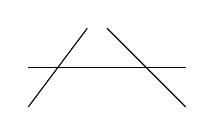
\begin{tikzpicture}
	\draw[name path=A] (0,0) -- (0.75,1)  (1,1)-- (2,0);

	\draw[name path=B] (0,0.5) -- (2,0.5);

	\pgfplotsfillbetween[of=A and B,split, every even segment/.style={orange}]{red}
\end{tikzpicture}

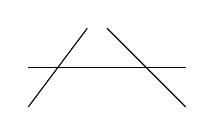
\begin{tikzpicture}
	\draw[name path=A] (0,0) -- (0.75,1)  (1,1)-- (2,0);

	\draw[name path=B] (0,0.5) -- (2,0.5);

	\pgfplotsfillbetween[of=A and B]{red}
\end{tikzpicture}
\end{document}

